\chapter{Durchführung}\label{sec:durch}

  Im anschlie{\ss}ende Abschnitt wird der Aufbau, sowie die Durchf\"uhrung und die Messmethodik des Experiments dieser Arbeit umrissen. Es folgt eine vertiefenden Beschreibung der Plasmakammer, einschlie{\ss}lich der Kameraanordnung mit Beleuchtungslasern. Eine Betrachtung des sog. \tilt{Plasma-Glow} wird ebenso Teil dieses Abschnitts sein. Zus\"atzlich soll dabei die dreidimensionale Rekonstruktion der Partikelbewegungen aus den Kamerabildern kurz beschrieben werden.

    \begin{figure}[H]
      \centering
      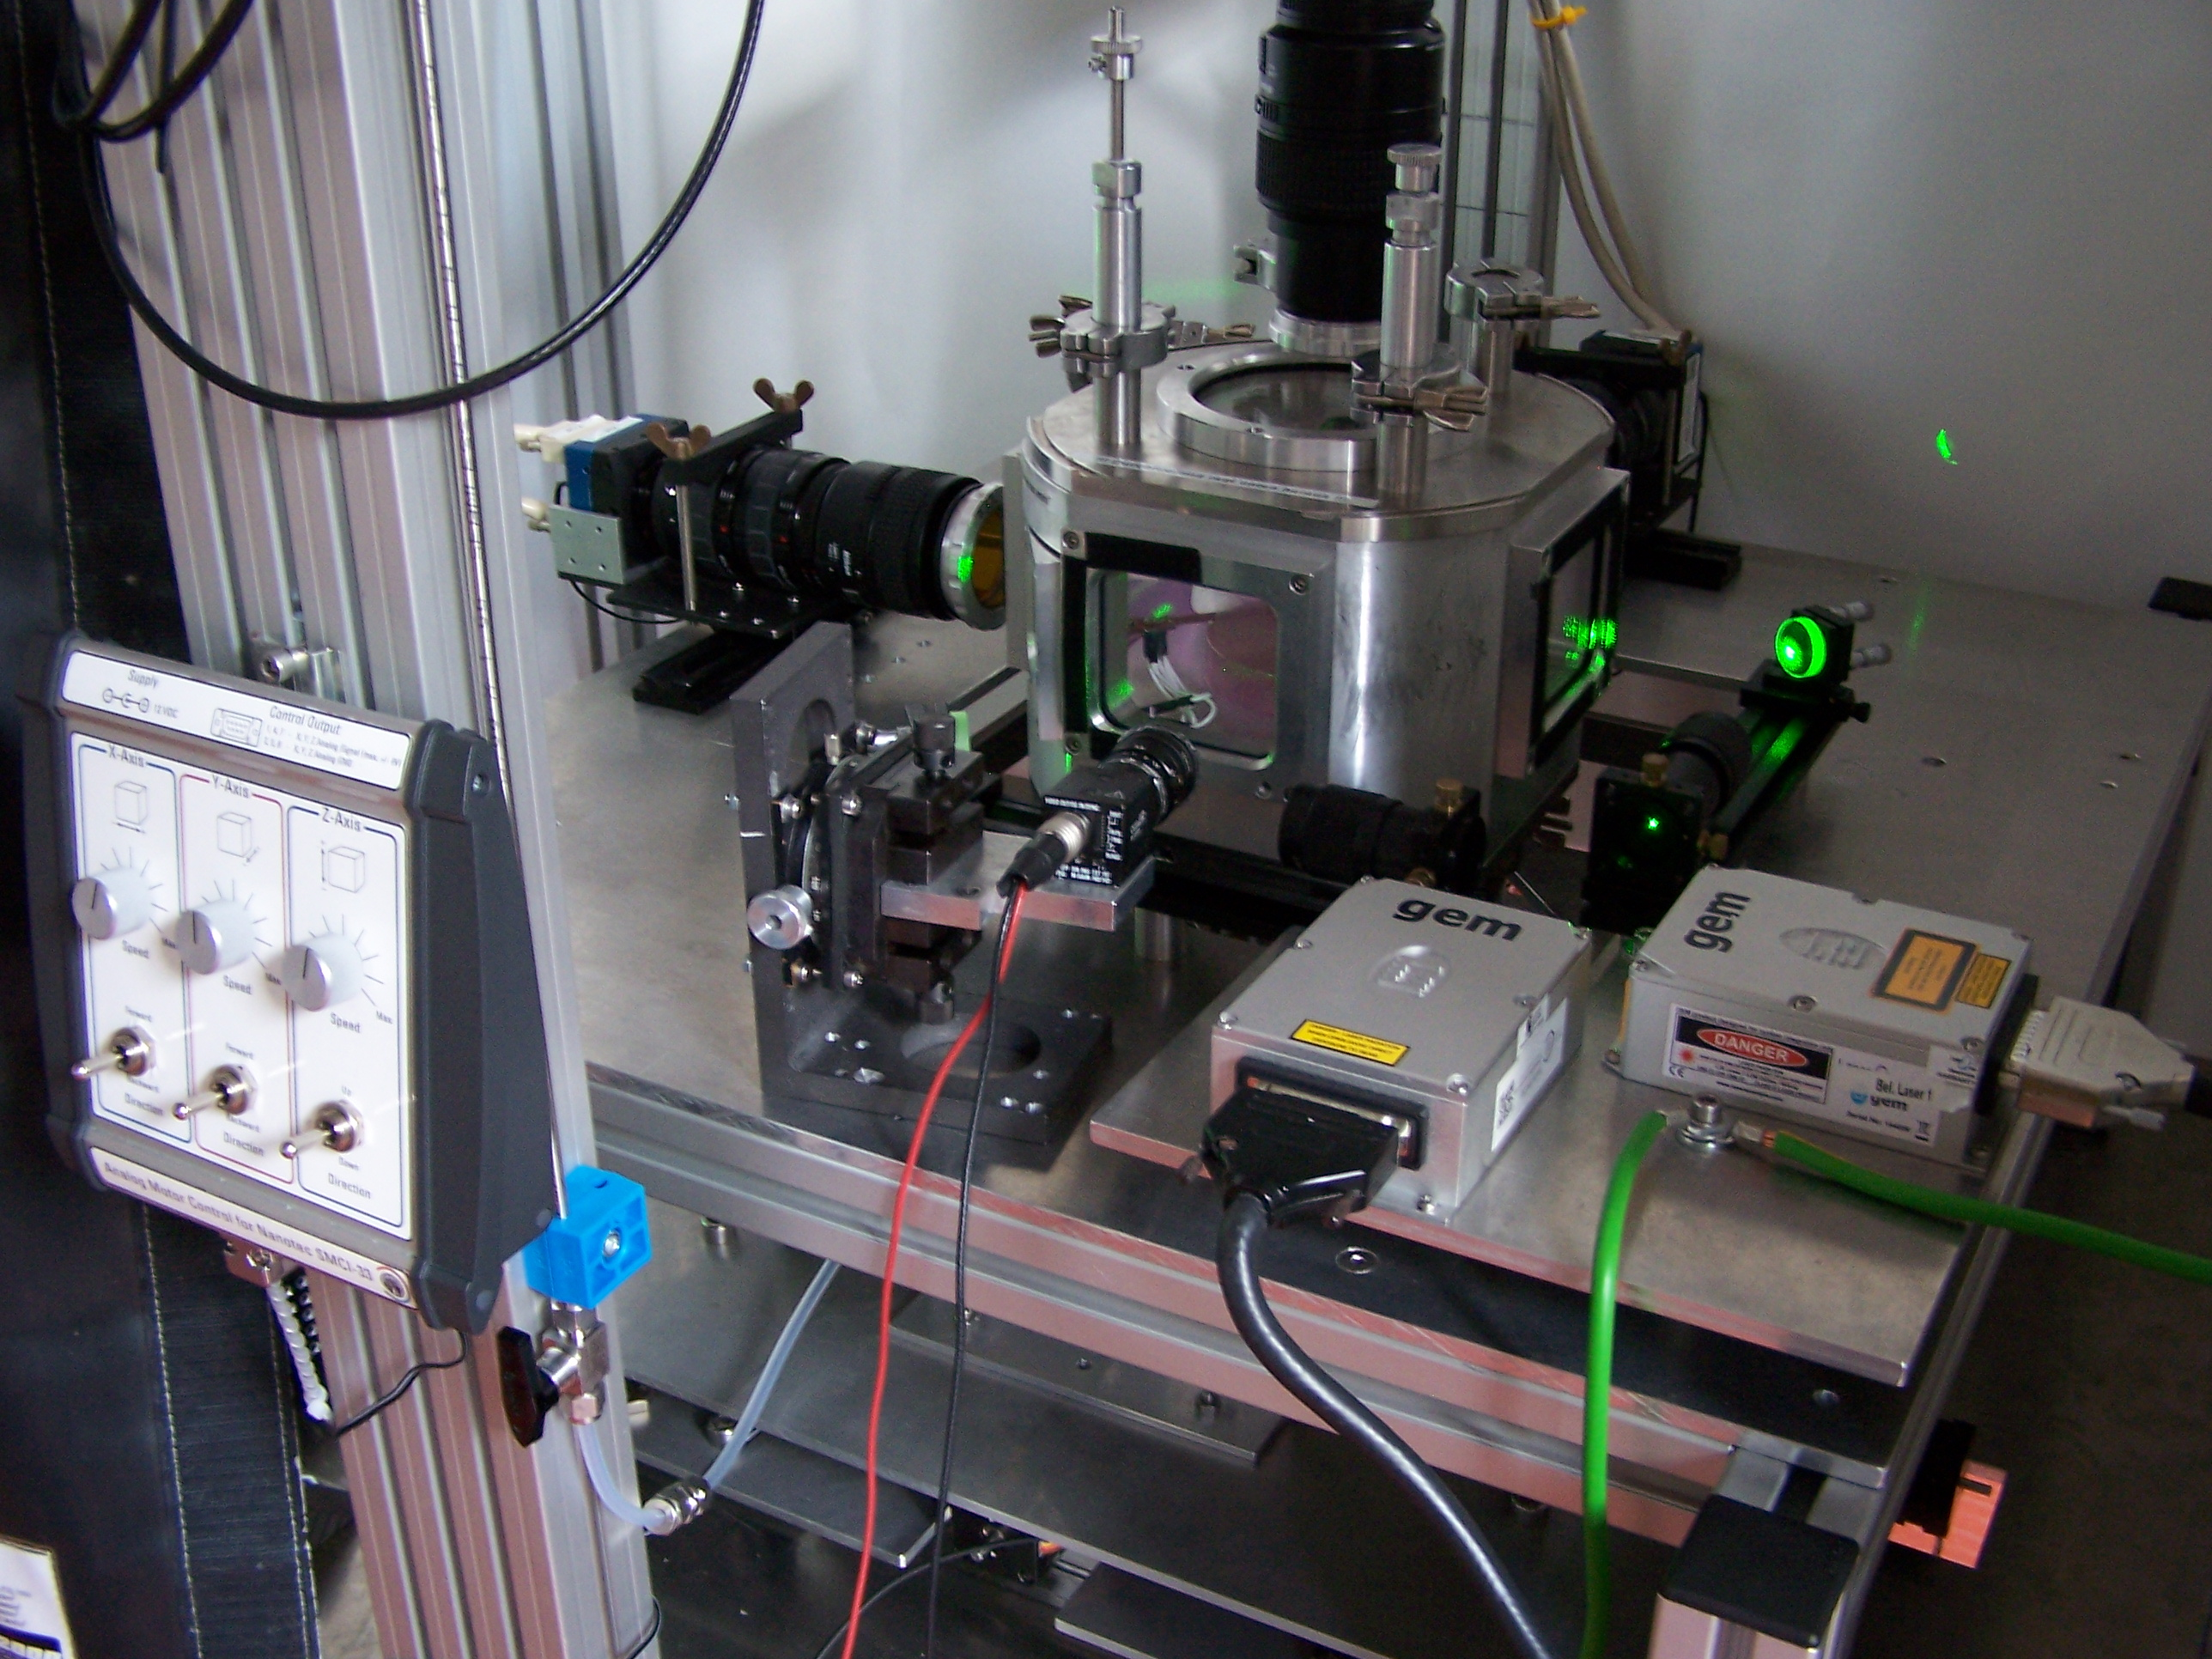
\includegraphics[width=\textwidth,height=0.7\textwidth]{figs/cam/aufbau.jpg}
      \caption{Versuchsaufbau bei eingeschaltetem Plasma mit grünen Beleuchtungslasern und verschiebbarem Tisch (siehe Steuerung links). Eine kleine Schwarz-Weiß-Übersichtskamera (Bildmitte vor der Kammer) ermöglichte auch bei laufendem Experiment die Beobachtung des Kammerinneren. Um den Versuch herum befand sich, als Sicherheitsvorkehrung, ein Laserschutzvorhang (Hintergrund).}
      \label{img:photo}
    \end{figure}

  \section{Aufbau}

      \begin{figure}[!t]
        \centering
        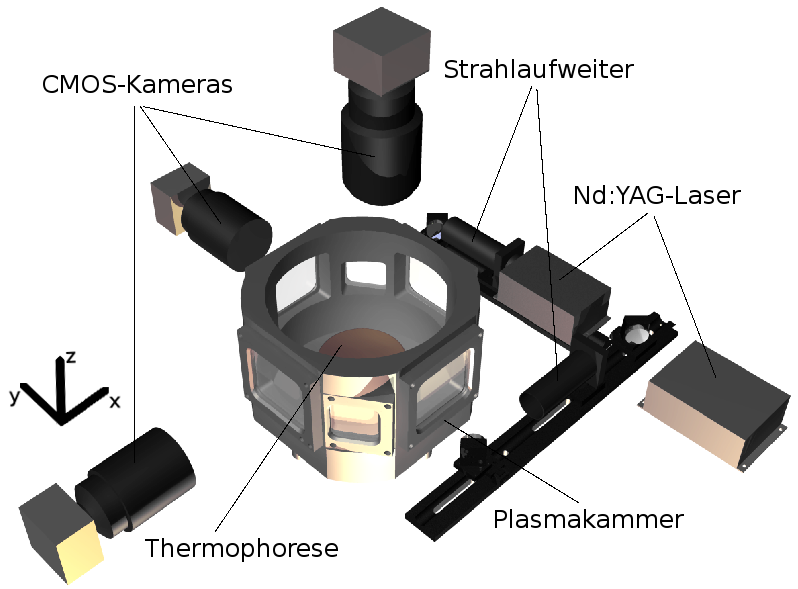
\includegraphics[width=0.75\textwidth,height=0.55\textwidth]{figs/witharrowsnunu.png}
        \caption{Schematische Ansicht des Stereoskopiesystems aus \autoref{img:photo}. Das eingezeichnete Koordinatensystem (rechts unten) entspricht dem der Tischbewegung und der späteren Auswertung (nach \cite{Mulsow13}).}
        \label{img:plasmakammer}
      \end{figure}

    Die in diesem Experiment verwendete Plasmakammer ist in \autoref{img:plasmakammer} gezeigt. Den fertigen Aufbau, samt Beleuchtungslaser und elektrisch verschiebbaren Versuchstisch zeigt das Photo in \autoref{img:photo}. Die Kammer hat einen Innendurchmesser von $\unit[25]{cm}$, wobei deren Deckel und Boden aus Edelstahl und die Wände aus Aluminium bestehen. Vier gro{\ss}e und 2 kleine, seitlich angebrachte, antireflexbeschichtete Fenster erm\"oglichen,  aus der Ebene den Blick auf den Yukawa-Ball. Im Deckel der Kammer befindet sich ein weiteres, kreisrundes Fenster mit einem Durchmesser von etwa $\unit[9]{cm}$. Die Beobachtung der Cluster wird durch drei zueinander orthogonale Kameras realisiert, wobei diese durch die genannten Glas-Einsätze in der Kammer schauen. Das daraus entstehende stereoskopische System nutzt man letztendlich zur Rekonstruktion der Teilchentrajektorien in 3D.\\
    Wie im Abschnitt \ref{sub:kaprfplasm} beschrieben, wird in diesem Versuch ein kapazitiv gekoppeltes Niederdruck-Radiofrequenz-Plasma in einer asymmetrischen Entladungskammer erzeugt. Eine abgeschirmte Messingelektrode befindet sich im unteren Teil des Aufbaus und wird, \"uber die kapazitive Kopplung zur Anpassung von Gleistromanteilen, von einem Generator mit einer Leistung zwischen $\unit[1-3]{W}$ bei einer Frequenz von $\unit[13,56]{MHz}$ betrieben. Der \"ubrige Teil der Kammer liegt auf Massepotential und dient damit als, fl\"achenm\"a{\ss}ig um ein vielfaches gr\"o{\ss}ere Gegenelektrode. \"Uber eine Pumpe wird die Kammer bis auf einen Restdruck von etwa $\unit[\tenpo{-1}]{Pa}$ evakuiert, damit sie m\"oglichst frei von Umgebungsluft ist und anschlie{\ss}end eine Argon-Entladung bei $\unit[5-12]{Pa}$ erzeugt werden kann.
    Weiterhin befinden sich im Deckel der Kammer Durchf\"uhrungen f\"ur den Staub aus MF (Melamin-Formaldehy) - $\unit[4,86\pm0,07]{\upmu m}$ im Radius - und die Einfang-Elektrode. Die Partikel werden \"uber ein Reservoir der Gr\"o{\ss}e eines 1 Cent-St\"uckes mit einer $\unit{\upmu m}$-gro{\ss}en Bohrung in die Entladung eingebracht. Die Befestigung der Ring-Elektrode aus \autoref{img:eingefangenerball} ist h\"ohenverstellbar und l\"asst sich leicht drehen, damit eine optimale Positionierung des Cluster in der Randschicht \"uber der getriebenen Elektrode bzw. der Thermophorese-Zelle vorgenommen werden kann.\\
    Die für den Einfang der Cluster genutzten Segmentringe (wie der in \autoref{img:ring} aus Abschnitt \ref{sub:einfang}) sind \"uber Koaxialkabel und eine weitere, unten liegende Vakuum-Durchf\"uhrung (4- bzw. 8-polig) mit der Manipulationselektronik verbunden. Genauer ist damit ein PC mit einer externen \fett{National Instruments 6364}-Karte, welche via USB und das Programm \fett{LabView} angesteuert wird, gemeint. Das erm\"oglicht es, verschiedenste Signale auf die einzelnen Bereiche der Elektrode zu bringen und damit das System gezielt zu heizen bzw. Moden anzuregen (siehe \autoref{img:ring}). 

      \begin{figure}[!t]
        \begin{subfigure}[t]{0.48\textwidth}
          \centering
          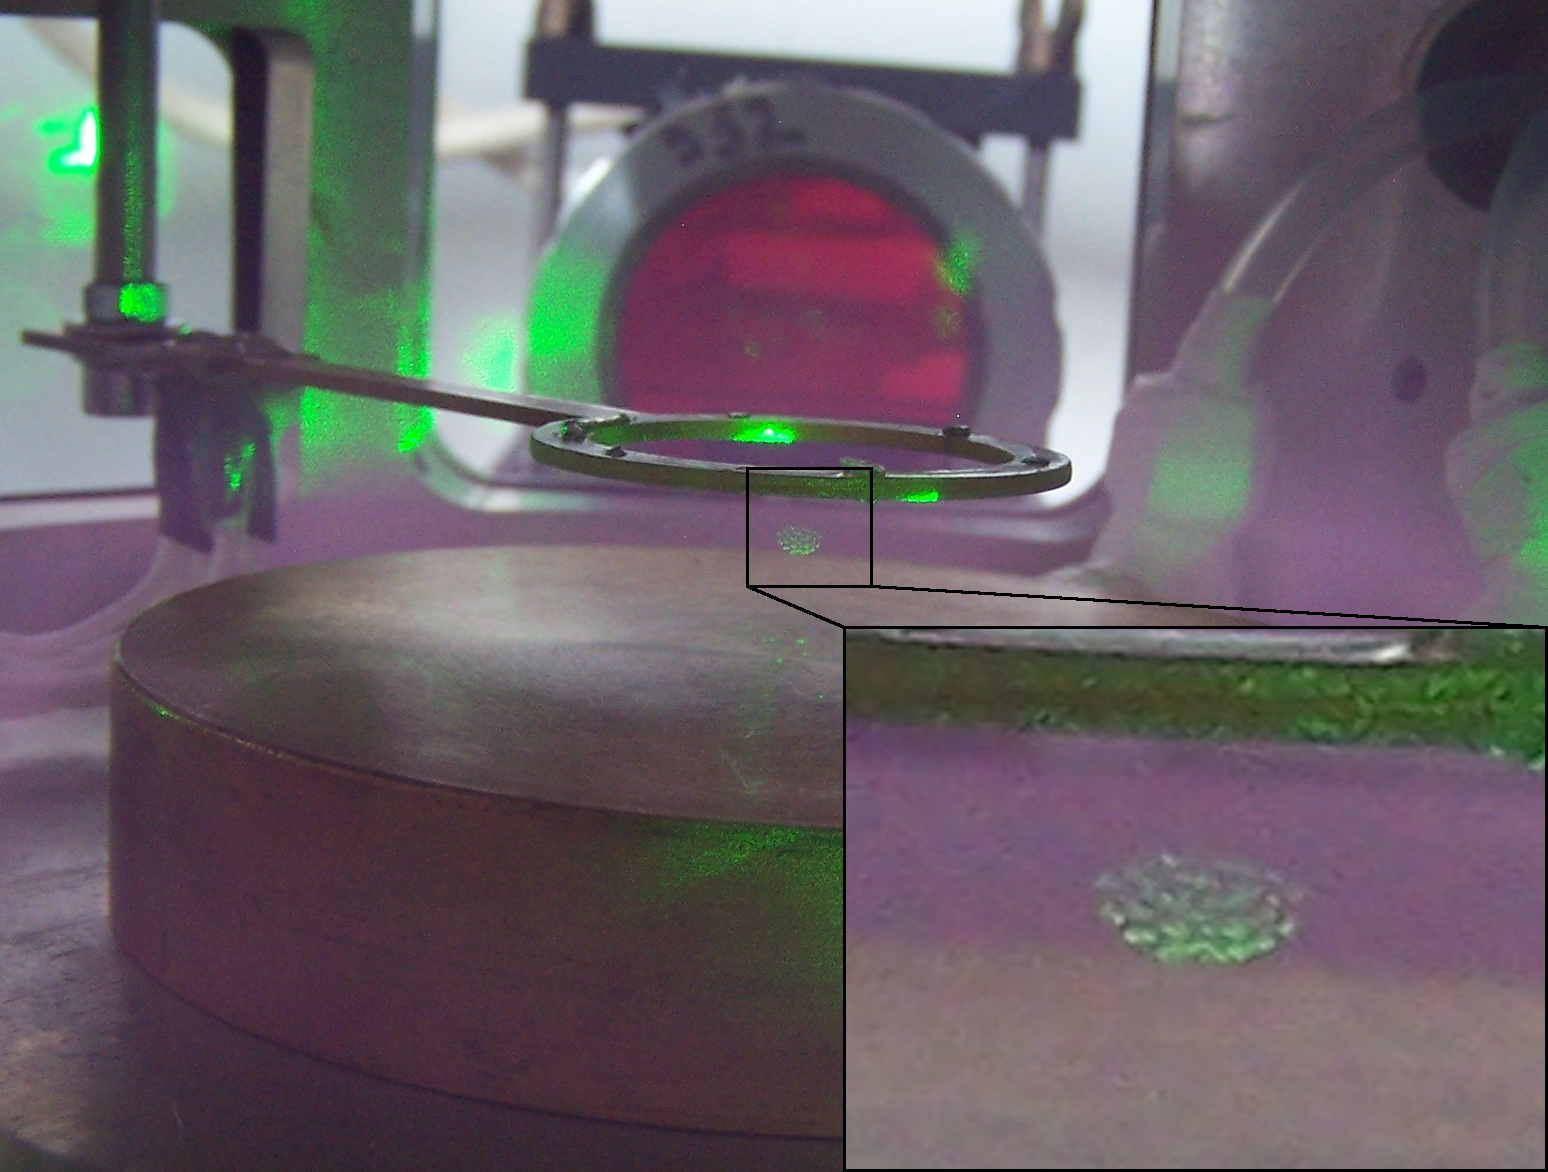
\includegraphics[width=\textwidth,height=0.75\textwidth]{figs/cam/innenansicht.jpg}
          \caption{}
          \label{img:eingefangenerball}
        \end{subfigure}
        \begin{subfigure}[t]{0.48\textwidth}
          \centering
          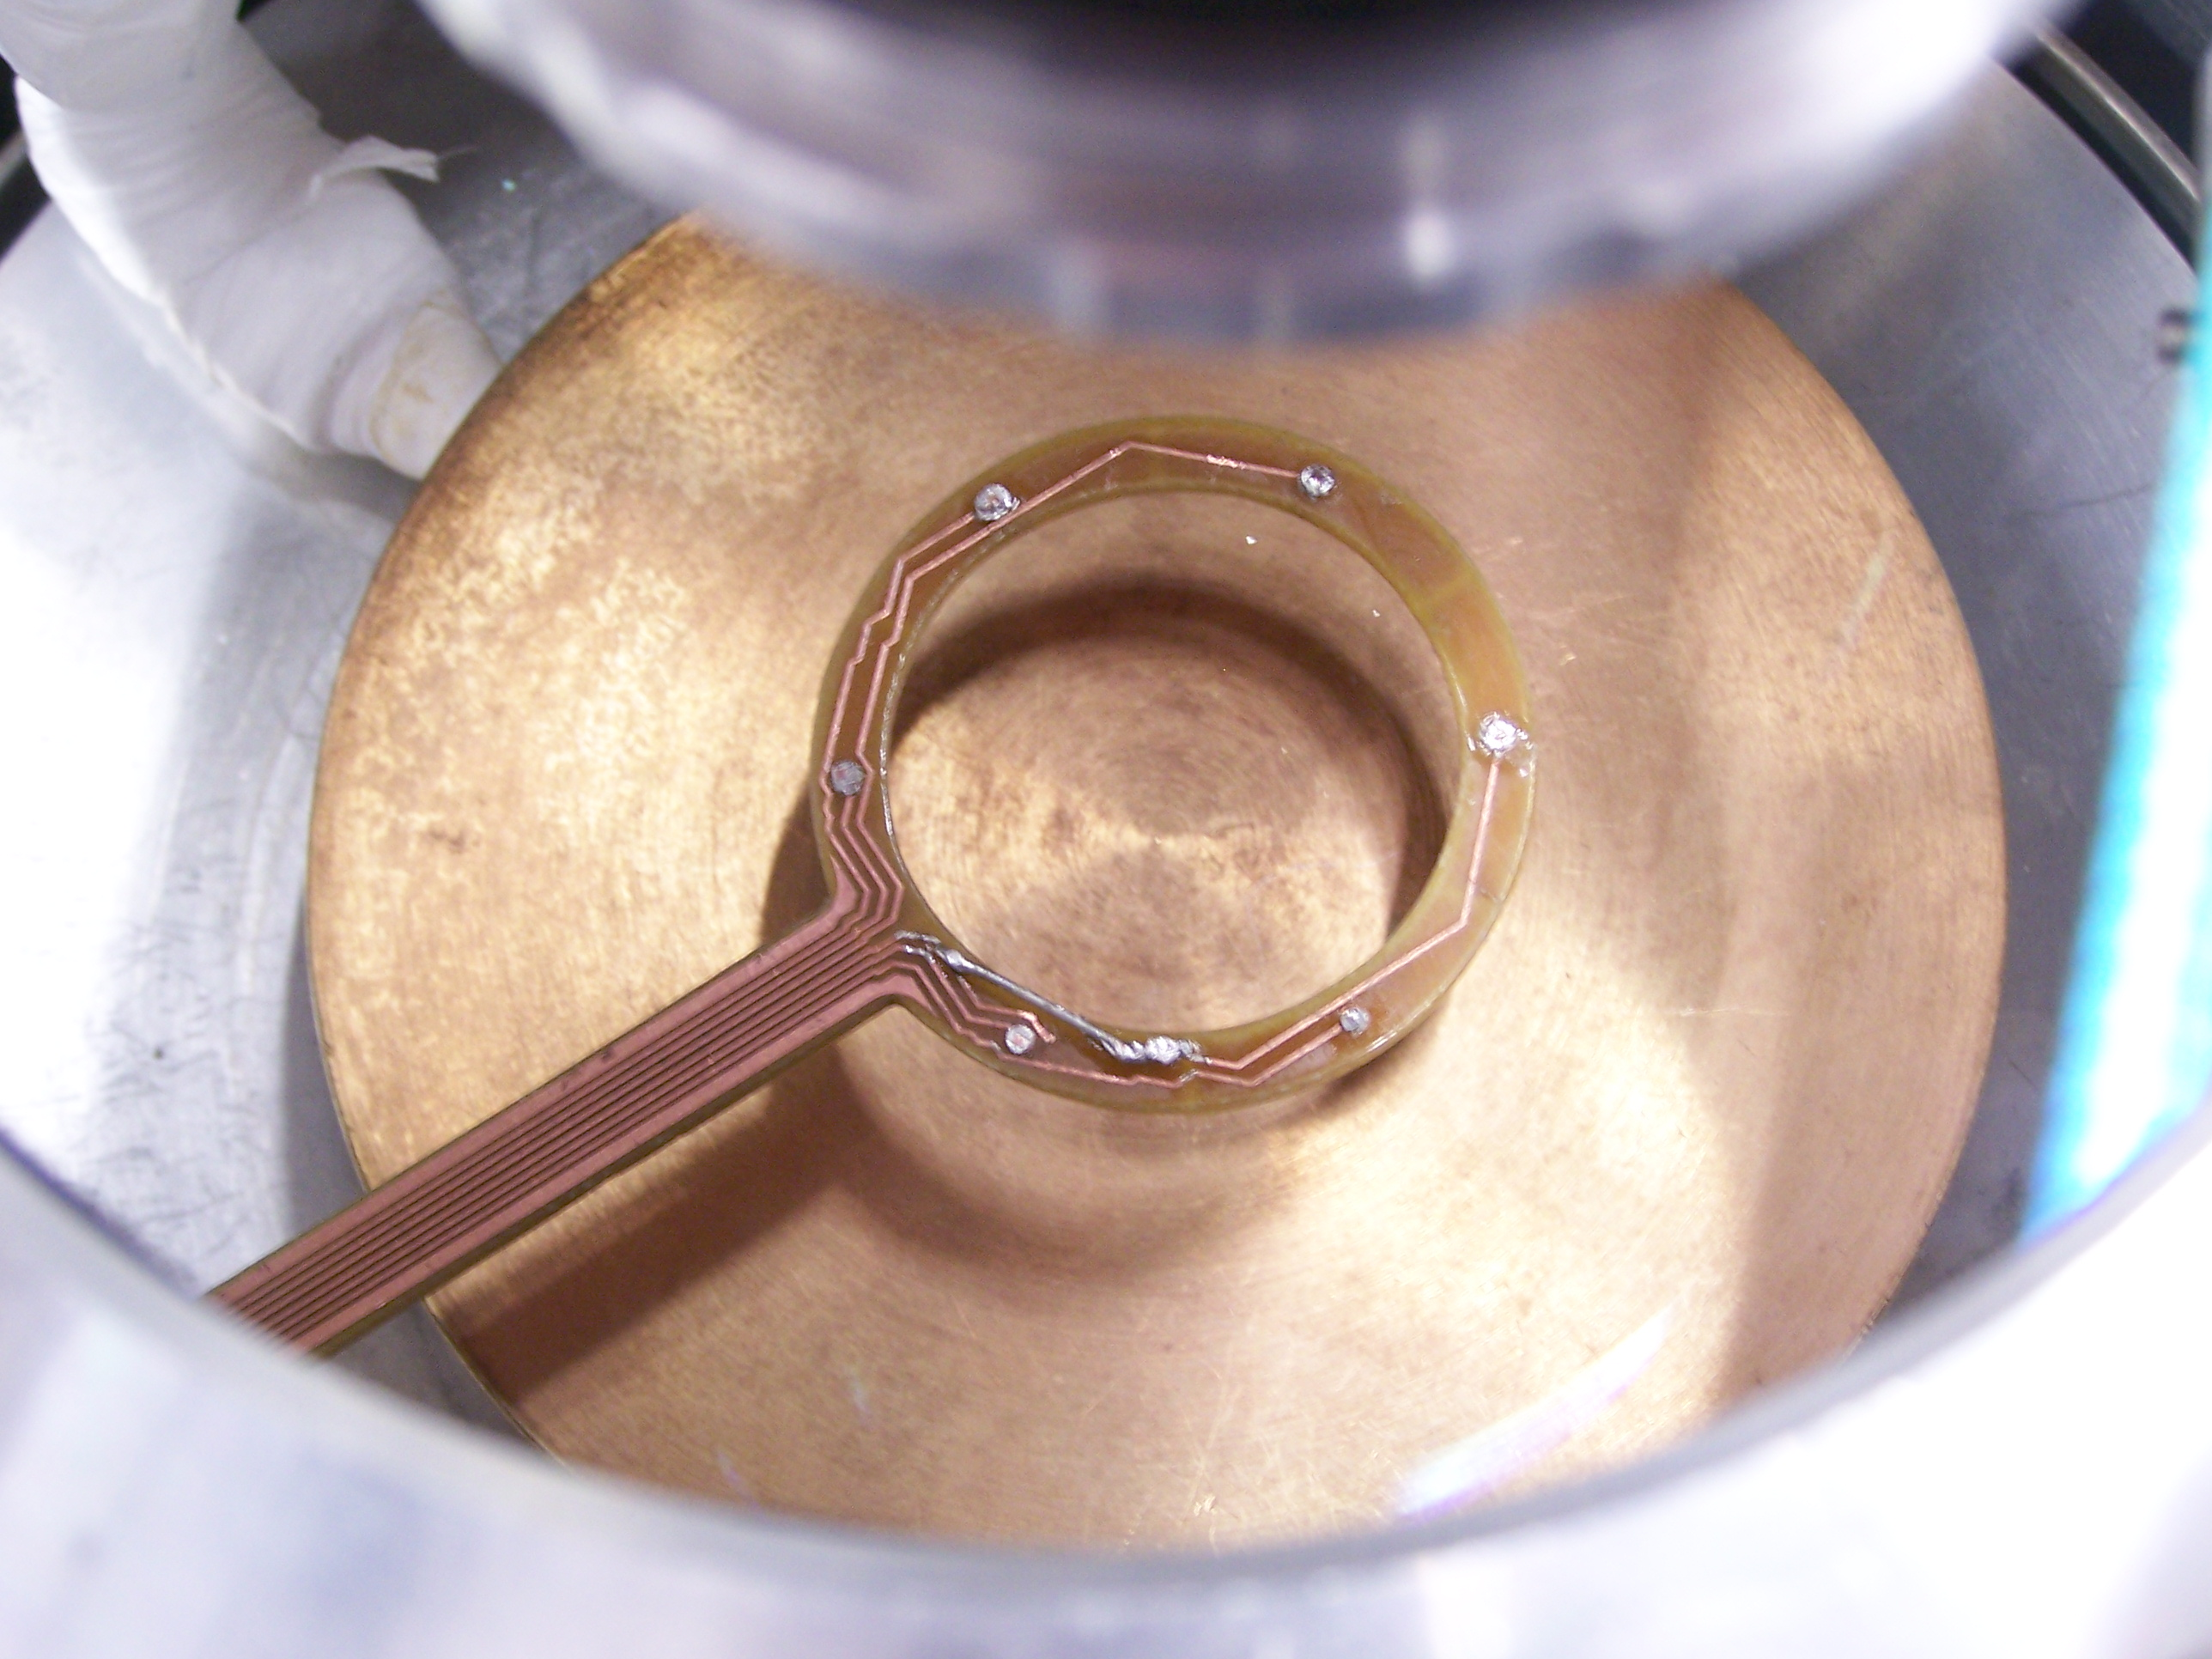
\includegraphics[width=\textwidth,height=0.75\textwidth]{figs/cam/topview.jpg}
          \caption{}
          \label{img:topview}
        \end{subfigure}
        \caption{\fett{(a)}: Einfang eines Yukawa-Balls mit $N\approx40$ unter Beleuchtung mit Nd:YAG-Lasern. Der Cluster befindet sich, leicht abhängig von der Höhe des Rings in der Randschicht, circa $\unit[0,5-1]{cm} $ unterhalb der Elektrode. Im Hintergrund: Kamera 'rot' mit Filter für $\unit[532]{nm}$. \fett{(b)}: Draufsicht durch den Deckel der Kammer auf den Ring. Günstiger Weise befindet sich dieser in der Mitte der Thermophorese, damit aus Sicht des, relativ dazu kleinen Clusters, die Randschicht unendlich ausgedehnt ist.}
      \end{figure}

  \section{Elektrischer Einfang} \label{sub:einfang}

      \begin{wrapfigure}{r}{0.5\textwidth}
        \centering
        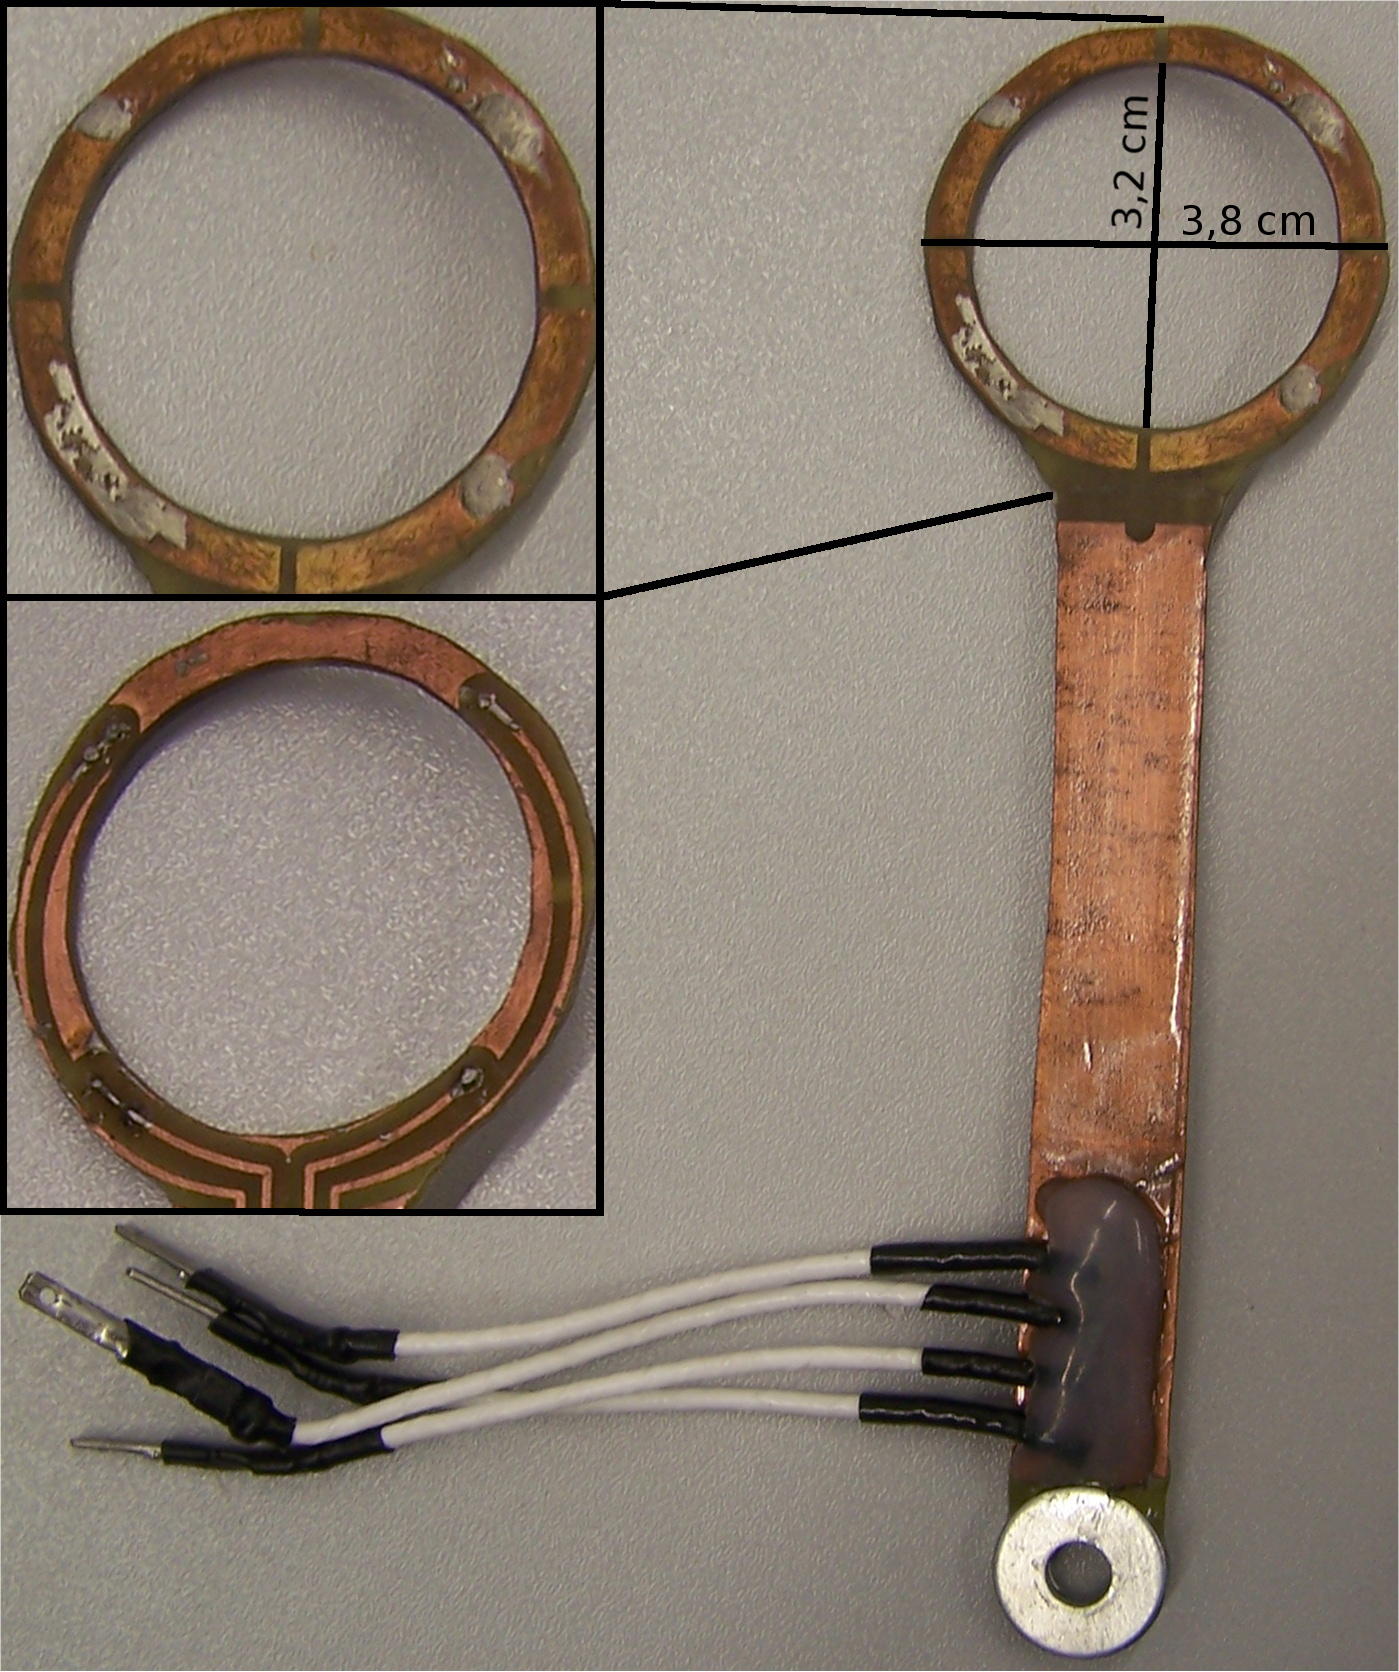
\includegraphics[width=0.45\textwidth,height=0.58\textwidth]{figs/cam/ringelektrode.jpg}
        \caption{Kupferring mit 4 Segmenten \underline{nach} der Benutzung (trotz Plastikumhüllung zeigt der Ring starke Abnutzungen durch Plasma). Am unteren Ende sind die weißen Vakuumkabel zu sehen.}
        \label{img:ring}
        \vspace{-0.5cm}
      \end{wrapfigure}

    Hauptaugenmerk dieses Experiments ist die Manipulation finiter Yukawa-Systeme. Hierf\"ur wurden eigens mehrsegmentige Kupferplatinen konzipiert und konstruiert, siehe \autoref{img:ring}. Deren - auf Skalen des Clusters- globaler Einflu{\ss} auf die Randschicht, welchen sie durch ihre zusätzlichen Potentiale erwirken, erm\"oglicht den Einfang eines Staubballs bei niedrigen Gasdr\"ucken und Plasmaleistungen. Weiterhin ist die Geometrie der Ring-Elektrode besonders g\"unstig f\"ur das vorliegende System, da sich somit ein sehr homogenes, sich der Symmetrie des Clusters angepasstes Einfangpotential einstellt.\\
    Die verwendeten Ring-Elektroden bestehen aus einem $\unit[6]{mm}$ starken, $\unit[3,2]{cm}$ im Inneren messenden Ring mit 4, 6 oder 8 Segmenten aus Kupfer an der Unterseite, welche später in Richtung des Clusters in der Randschicht zeigen. Dieser Ring ist mit einem Arm, über den die Leiterbahnen der jeweiligen Segmente laufen, verbunden. Am Ende dessen befindet sich eine Bohrung, durch welche die Durchführung mit Schraubgewinde im Kammerdeckel geführt werden kann und somit die Positionierung bei geschlossenem Aufbau ermöglicht. Die gelöteten Kontaktierungen der Vakuumkabel für die Manipulation, von der Ober- auf die Unterseite führend, liegen knapp vor der Bohrung. Für einen Vergleich siehe \autoref{img:ring}, sowie  \autoref{img:eingefangenerball}  und \autoref{img:topview}. Ziel der Manipulation durch die segmentierte Ring-Elektrode ist es, verschiedene Moden mit unterschiedlichen Symmetrien - Dipol, Quadrupol usw. - gezielt anzuregen und in diese Energie zu bringen. Durch die Modentheorien aus Abschnitt  \ref{sub:yukawaclust} und deren Ausdrücke für die Energie pro Mode $Q_{lm}\left(\omega\right)$ bzw. $S\ix{p}\left(\omega\right)$ kann danach bestimmt werden, inwiefern die Störung erfolgreich war und welche Konsequenz dies nach sich zieht. Auf die Veränderung der Randschicht durch den Ring wird in \ref{sub:glow} eingegangen.


  \section{Strereoskopie und Bildrekonstruktion}

    Die Zeitskala der Dynamik der Staubteilchen erlauben eine strereoskopische Untersuchung des Systems. Die Beobachtung erfolgte \"uber 3, zueinander orthogonale High-Speed-CMOS-Kameras mit 60 bzw. $\unit[105]{mm}$ Objektiven. Deren Aufnahmen von bis zu 500 Bildern pro Sekunde ($\unit{fps}$ - \tilt{frames per second}) haben eine maximale Aufl\"osung von $\unit[1280\times1024]{px}$. Dabei nimmt die \tilt{fps}-Zahl mit steigender Auflösung ab: je mehr Daten aufgenommen und verarbeitet werden müssen, umso niedriger ist die maximale, verlustfreie Aufnahmerate.\\
    Für die Messreihen wurden jeweils Bilderserien von 10000 \tilt{frames} aufgenommen, wobei die Geschwindigkeit sich dem zu untersuchenden Sachverhalt anpasste. F\"ur eine "`freie"' Aufnahme lag diese bei 100 Bildern pro Sekunde: der Cluster war entweder ungest\"ort oder wurde bei einer festen Anregungsfrequenz manipuliert. Waren Informationen zu bestimmten Phasen gesucht, so wurde dementsprechend die Kamera mit der Anregung gekoppelt und dabei 4 Bilder pro Periode bei einer Frequenz von bis zu $\unit[6,5]{Hz}$ gemacht. \\
    Beleuchtet wurde der Yukawa-Ball mit 2 gr\"unen Nd:YAG-Lasern, welche bei einer Wellenl\"ange von $\unit[532]{nm}$ und mit einer Leistung von $\unit[600]{mW}$ abstrahlten. Über Strahlaufweiter und Spiegel wurden die Laser diagonal durch die Entladung geleitet (siehe \autoref{img:eingefangenerball}). Strahlprofil und Strahlungsdruck (siehe \ref{subsub:laser}) sind durch diesen Aufbau so konstruiert, dass sie f\"ur die Dynamik des Clusters unkritisch sind. Jedoch beobachtet man bei an- und ausschalten der Laser eine Verschiebung des Clusters. In \cite{Mulsow13} sind tiefgreifendere Untersuchungen zur Manipulation mit Lasern vorgenommen worden.\\
    Da die Ausdehnung der Partikel weniger als $10\cdot\lambda$ des Laserlichts ist (siehe \cite{Mie08} o. \cite{Hulst81}), kann zur Beschreibung des Streuverhaltens der Staubteilchen die Mie-Streuung herangezogen werden (\cite{Bonitz10}). Nach dieser Theorie ist das vorw\"arts gestreute Licht am intensivsten. Deswegen befinden sich die Kameras auf den gegen\"uberliegenden Seiten der Punkte, an denen das Laserlicht eingestrahlt wird: es resultiert ein kontrastreiches Bild, auf welchem die Partikel gut vor dem dunklen Hintergrund zu sehen sind (siehe \autoref{img:rechts} und weitere). Damit einher gehen jedoch auch Probleme, wie zum Beispiel das es zu einer \"Uberbelichtung oder Komplikation bei der Ausrichtung des Systems aus Cluster, Elektrode, Laser und Vakuumkabel kommen kann.

%			Die Bildverarbeitung erfolgte im graustufigen \tilt{bitmap}-Format, kurz \tilt{*.bmp}. Dabei handelt es sich um ein zweidimensionales Rastergrafikformat, bei dem, wie in einer Matrix, einem Pixel die Graustufen-Information mit einem 8-Bit-Wert zugeordnet wird. Das erleichterte u.a. die Verarbeitung in Hinblick auf Intensit\"atsanalysen, wie die Partikelerkennung oder die Auswertung des Plasma-Glow (siehe \ref{sub:glow}).
          
              \begin{figure}
                  \begin{subfigure}[b]{0.4\textwidth}
                      \centering
                      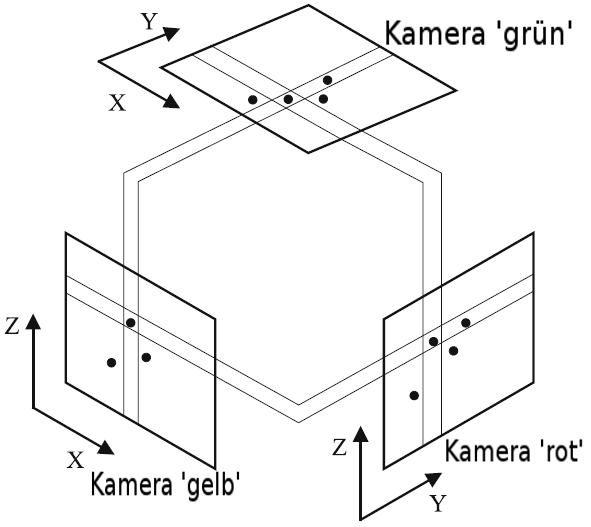
\includegraphics[width=\textwidth,height=5.5cm]{figs/rekonstruktion.png}
                      \caption{}
                  \end{subfigure}
                  \begin{subfigure}[b]{0.56\textwidth}
                      \centering
                      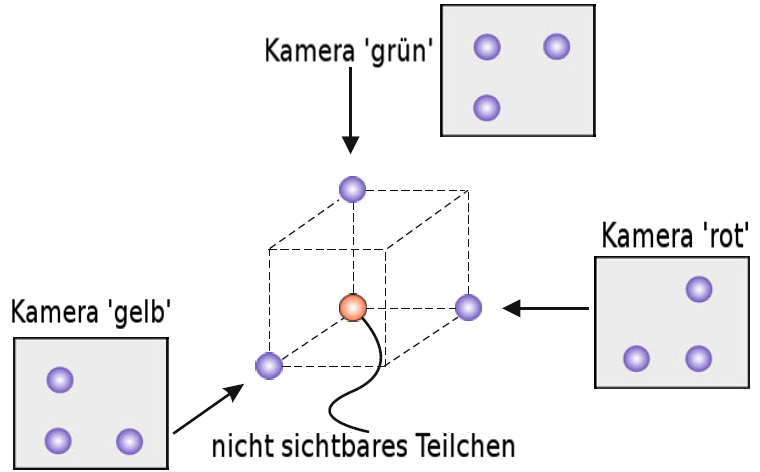
\includegraphics[width=\textwidth,height=5.5cm]{figs/nichtsichtbar.png}
                      \caption{}
                  \end{subfigure}
                  \caption{\fett{(a)}: Rekonstruktion der dreidimensionalen Informationen aus den Bildern der Kameras. \fett{(b)}: Fehler in der Analyse durch Überlagerung von 4 Teilchen in drei Bildern. Für kurze Zeiten des 'Verschwindens' kann mittels Interpolation die Trajektorie des nicht sichtbaren Teilchens vervollständigt werden (nach \cite{Bonitz10}).}
                  \label{img:rekonstruktion}
              \end{figure}

      \subsection{3D-Trajektorien}

        Die Rekonstruktion der dreidimensionalen Informationen des Beobachtungsvolumen ist das Kernst\"uck der Stereoskopie (\cite{Bonitz10}). Eingangs m\"ussen aus den einzelnen \tilt{frames} der Kameras die Partikelpositionen gewonnen werden. Daf\"ur analysiert man das Bild durch einen (\tilt{gau{\ss}schen}) Bandpass der Breite des erwarteten Partikeldurchmessers (\cite{Crocker96a}, \cite{Ivanov07}). Au{\ss}erhalb liegende Objekte werden gegl\"attet und angepasst. F\"ur alle erkannten Teilchen wird anschlie{\ss}end, der Intensit\"atsverteilung \"uber diese entsprechend, deren Schwerpunkt ermittelt. Damit erhält man eine Auflösung im Sub-Pixel-Bereich. Es ergeben sich f\"ur alle Kameras die zweidimensionalen Informationen \"uber Partikelpositionen und Clusterausdehnung.\\
        Die Zuordnung der Partikel in gleichzeitigen Kamera-Bildern ist in \autoref{img:rekonstruktion}:\fett{(a)} schematisch dargestellt. F\"ur jeden Augenblick der Aufnahme stimmt eine Koordinate der gewonnenen Tupel (eines Partikels) mit einer in den anderen beiden zugeh\"origen \tilt{frames} \"uberein. Dies gilt gerade aufgrund der Orthogonalität des Systems. Durch Abgleich der Informationen von jeweils 2 Kameras und deren Kombination, kann aus den zwei- die dreidimensionalen Koordinaten der Teilchen gewonnen werden. Die letztendlich erhaltenen Partikel-Trajektorien ergeben sich durch die Verknüpfung der \tilt{nearest neighbors} in zwei aufeinander folgenden Bilder. Das heißt, dass die Zusammenführung der Teilchenkoordinaten aus den Aufnahmen zweier Kameras für einen weiteren Zeitschritt fortgesetzt wird. Es wird das Intensitäts-Maximum mit dem kleinsten Abstand zum Ort des betrachteten Partikels im vorherigen Bild gesucht und folglich mit diesem zum entsprechenden Zeitpunkt identifiziert. Die damit erhaltenen Punkte der Bewegung für die diskreten Zeiten der Aufnahme ergeben die Trajektorie.
        Die Rekonstruktion mittels 3 Beobachtungsrichtungen senkt dabei die Wahrscheinlichkeit, dass aufgrund der thermischen Bewegung oder Manipulation (ggf. auch Clusterkonfiguration) Partikel hintereinander verschwinden und somit nicht mehr durchg\"angig aufgenommen werden k\"onnen (siehe \autoref{img:rekonstruktion}:\fett{(b)}). F\"ur einzelne Bilder, in denen sich Partikel \"uberdecken, lassen sich jedoch die Trajektorien durch Interpolation, was u.U. f\"ur Fehler in der Auswertung auf Grund von Artefakten sorgen kann, vervollst\"andigen.

  \section{Analyse des Plasma-Glow} \label{sub:glow}

  Im Zuge der Untersuchung einer Quadrupolschwingung bemerkt man leicht, dass die Teilchen des Clusters, zusätzlich zu ihrer Auslenkung in der Ebene, eine vertikale Schwingung mit Maximum zum Zeitpunkt des Nulldurchgangs der sinusoidalen Signale ausführen. Die Anregung dieser Mode enthält jedoch keine solchen Anteile. Diese Beobachtung legt demnach nahe, dass die Randschichtveränderung durch das Einfangpotential nicht vernachlässigbar für die Kinematik des Cluster ist.\\
  Aus den Abschnitten \ref{sub:kaprfplasm} und \ref{sub:rand} wissen wir,  dass sich beispielsweise um metallische Objekte in einem Plasma eine Grenzschicht ausbildet. Weiterhin ist deren Ausdehnung und Eigenschaften abhängig vom Potential des lokalen Plasmas bzw. des Objektes selbest. Deswegen ist die Manipulation eines Yukawa-Clusters nicht nur als elektrostatische Wechselwirkung Staub und Ring-Elektrode (siehe \autoref{img:potential}) zu verstehen, sondern viel mehr als Summe dessen und der Veränderung der lokalen

    \begin{wrapfigure}{l}{0.45\textwidth}
      \centering
      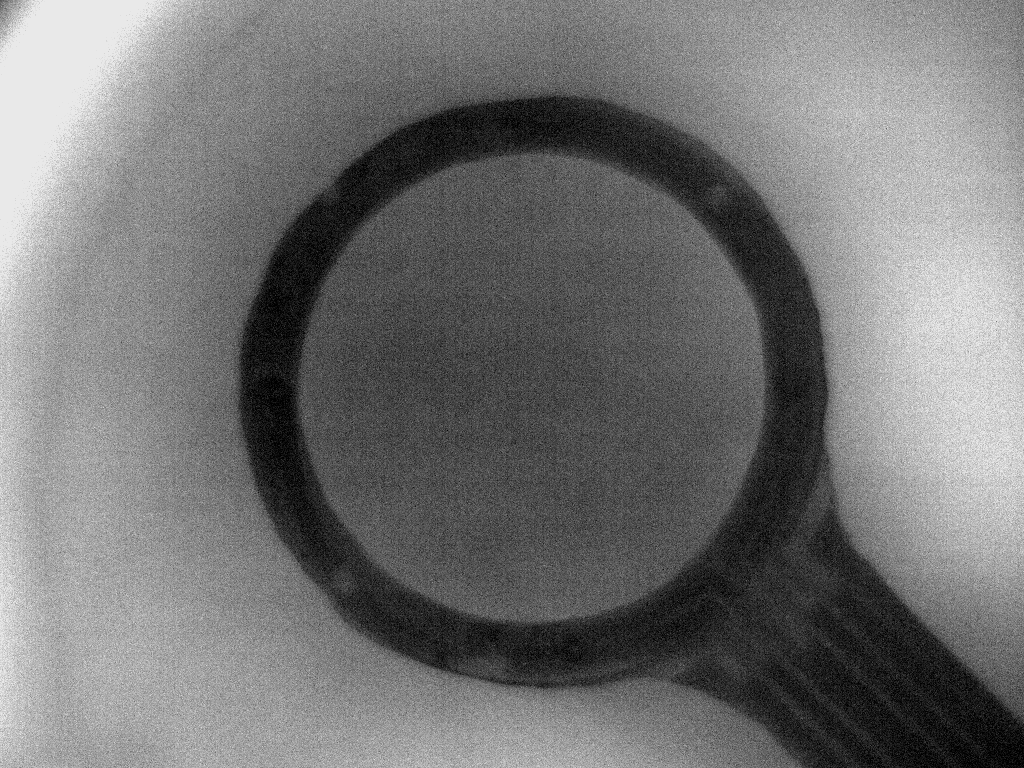
\includegraphics[width=0.4\textwidth,height=0.3\textwidth]{figs/ringplasmglowoben.png}
      \caption{Ein \tilt{frame} ohne Filter für das Licht der Argon-Entladung. Die Helligkeit in der Mitte ist geringer als außerhalb.}
      \label{img:glow}
      \vspace{-0.2cm}
    \end{wrapfigure}

  Randschicht, in welcher sich die Staubpartikel befinden. Letztendlich war der Einfang eines Staub-Balls als Balance mit der elektrischen Kraft zu verstehen, welche gerade durch das Feld in der Randschicht bei $\unit{\upmu m}$ bestimmt wurde. Ein Maß für ihre Ausdehnung, und somit daraus folgend ihre weiteren Eigenschaften, ist das Leuchten der Neutralgasatome des Argons. Dieses ist intensiver, je größer die vorliegende Elektronendichte und/oder -temperatur ist (siehe \ref{sub:rand}).  Auf Grund dessen erhält man aus einer Intensitätsanalyse des Bereiches aus \autoref{img:glow} Informationen über die Stärke der Randschichtveränderungen. Ohne die, während der restlichen Messungen an den Kameras angebrachten Filter für das Plasmaleuchten, wurden Aufnahmen für verschiedenste Anregungen gemacht. Das heißt: die 4 Segment des Ringes wurden, entsprechend der gewünschten Symmetrie, mit einer festen Phase zueinander und Frequenz mit einem sinusoidalen Signal der Amplitude $\unit[10]{V}$ beschaltet. Von Interesse sind dabei jedoch nur die Bilder der Oberkamera ('grün', siehe \autoref{img:glow}). Die \tilt{bitmaps} werden für die Analyse zuerst auf ein \tilt{range of interest} - ein Kreis bzw. eine Kreisscheibe, in welcher das Leuchten ausgewertet werden soll - beschnitten. Anschließend wird das \tilt{ROI} in Radius- und Winkelabschnitte eingeteilt, welche in ihrer Intensität aufsummiert werden.

%			\begin{figure}[!h]
%				\begin{subfigure}{0.49\textwidth}
%					\centering
%					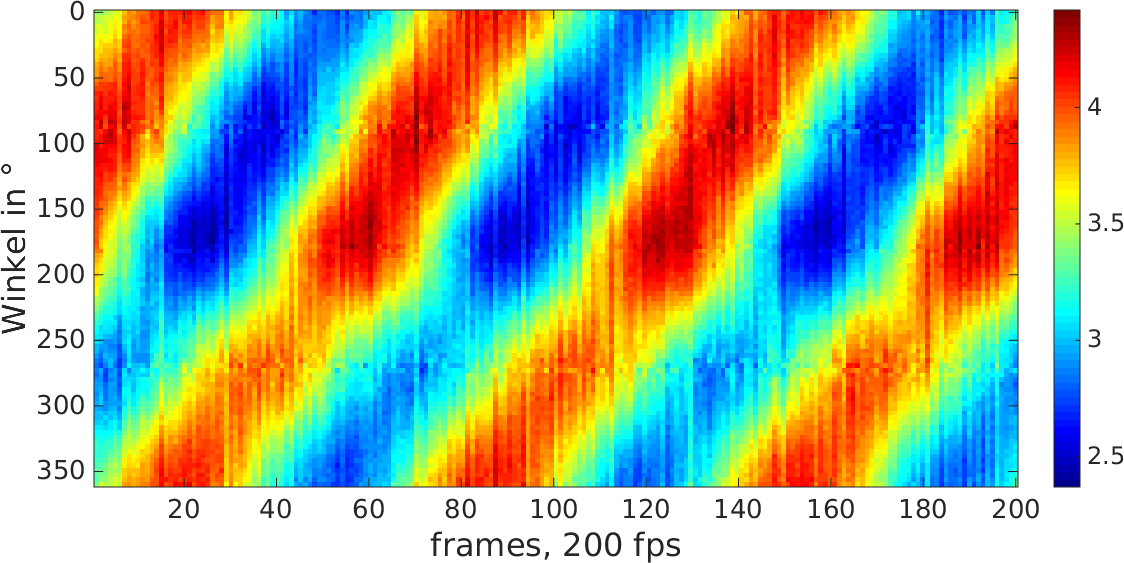
\includegraphics[width=\textwidth]{figs/glowbeispielrotation3Hzang.png}
%				\end{subfigure}
%				\begin{subfigure}{0.49\textwidth}
%				\centering
%				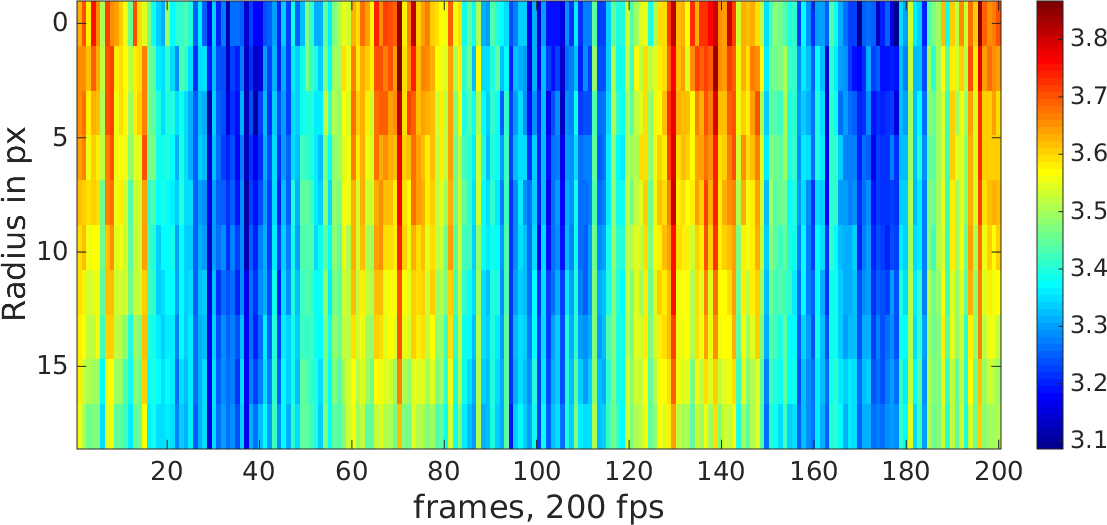
\includegraphics[width=\textwidth]{figs/glowbeispielrotation3Hzrad.png}
%				\end{subfigure}
%				\caption{\underline{\fett{links}}: Winkelaufgelöste Rotationsanregung ($\unit[3]{Hz}$, max. Amplitude). Bei $\unit[250]{\degree}$ ist eine Asymmetrie zu erahnen. \underline{\fett{rechts}}: Radiale Auflösung. Die Randschichtveränderung ist innen stärker als außen.}
%				\label{img:glowanalys}
%			\end{figure}

  \section{Phasenaufgelöste Aufnahme}\label{sec:phasen}

    Die Anregung über die Ring-Elektrode aus \ref{sub:einfang} ist sinusoidal. Die Kraft durch das zusätzliche Potential hat demnach die Form $F\ix{ext}=K\sin\left(\omega t\right)$, wobei $K$ eine kleine Amplitude ist und $\omega$ die Anregungsfrequenz. Da aus den bisherigen Überlegungen klar gorden ist, dass der Staub-Cluster Reibungskräfte erfährt, lässt sich dessen Schwingungsantwort $C\left(t\right)$ in Hinblick auf die Manipulation als, um den Faktor $\gamma$ gedämpfter, harmonischer Oszillator verstehen (siehe \autoref{eq:gedämpft} nach \cite{Carstensen11}). Außerdem ist aus Abschnitt \ref{subsub:moden} bekannt, dass das System ebenso eine Eigenfrequenz $\omega\ix{0}$ besitzt. Diese zu bestimmen ist u.U. sehr aufwändig, muss man doch bei kontinuierlichen Messungen für relativ große Zeiten beobachten, um schließlich für eine einzelne Frequenz die Resonanzantwort zu bestimmen. Geht man hingegen von den \autoref{eq:gedämpft} - (\ref{eq:amplitud}) aus, so reicht es, die Amplituden zu 4 verschiedenen Phasen - für $\phi\omega t=0\degree,90\degree,180\degree,270\degree$ verschwindet jeweils ein Teil in \autoref{eq:gedämpft} - aufzunehmen, um daraus schließlich $\omega\ix{0}$ zu errechnen.

      \begin{align}
        C\left(t\right)=a\left(\omega\right)\sin\left(\omega t\right)+&b\left(\omega\right)\cos\left(\omega t\right) \label{eq:gedämpft} \\
        a\left(\omega\right)=-\frac{K\left(\omega\ix{0}^2-\omega^2\right)}{\left(\omega\ix{0}^2-\omega^2\right)^2+\left(2\gamma\omega\right)^2} \quad& b\left(\omega\right)=-\frac{2K\gamma\omega}{\left(\omega\ix{0}^2-\omega^2\right)^2+\left(2\gamma\omega\right)^2} \\
        A\left(\omega\right)=\sqrt{a^2\left(\omega\right)+b^2\left(\omega\right)}=&\frac{K}{\sqrt{\left(\omega\ix{0}^2-\omega^2\right)^2+\left(2\gamma\omega\right)^2}} \label{eq:amplitud}
      \end{align}

\newpage

    Um eine phasenaufgelöste Aufnahme für verschiedene Frequenzen zu machen, wurde die Anregung an die Kameras als neuer Trigger gekoppelt. Das bedeutet, dass die Anregung einen digitalen Puls an die Kameras sendet, wenn sie die entsprechenden Phasen erreicht hat. Für einen Frequenzbereich von $1,6$ bis $\unit[6,5]{Hz}$, bei Inkrementen von $\unit[0,1]{Hz}$, wurden für jeweils 50 Schwingungen 4 Bilder gemacht. Die daraus erhaltenen Daten ergaben Graphen der Art von \autoref{img:amplitud}. Sie ergeben die Resonanz- und Eigenfrequenz der Systeme. Diese können dann mit den erhaltenen Daten zBsp. der Normalmoden-Analyse verglichen werden. Insbesondere liefert die Resonanzfrequenz Informationen über den Einfluss der Reibung auf die Schwingungen des Clusters.

      \begin{figure}[H]
        \centering
        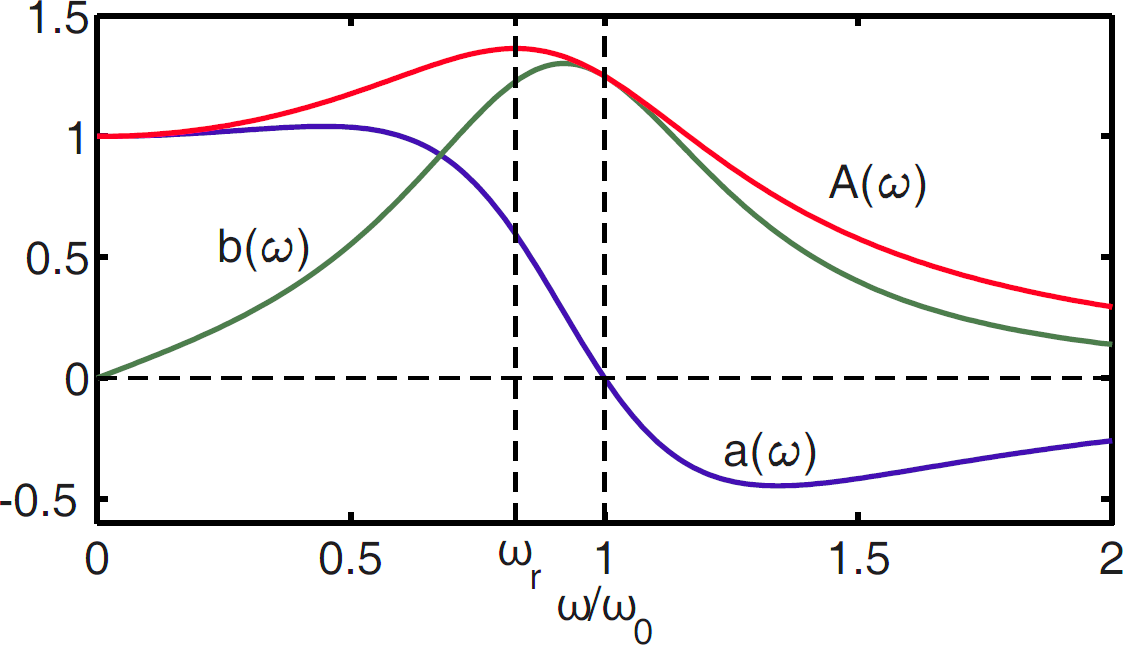
\includegraphics[width=0.7\textwidth,height=0.35\textwidth]{figs/amplitud.png}
        \caption{$A\left(\omega\right), a\left(\omega\right), b\left(\omega\right)$ normiert auf $\omega\ix{0}^2/K $ für $\gamma/\omega\ix{0}=2,5$. Der Wert $\omega\ix{r}$ ist die Resonanzfrequenz, an welcher die Schwingunsantwort die größte Amplitude hat (nach \cite{Carstensen11}).}
        \label{img:amplitud}
      \end{figure}

